\documentclass[
  shortnames]{jss}

%% recommended packages
\usepackage{orcidlink,thumbpdf,lmodern}

\usepackage[utf8]{inputenc}

\author{
Gilberto Camara~\orcidlink{0000-0002-3681-487X}\\Nat Inst for Space Research\\
Brazil \And Rolf Simoes~\orcidlink{0000-0003-0953-4132}\\Nat Inst for Space Research\\
Brazil \And Renato Assunção~\orcidlink{0000-0001-7442-9166}\\Federal Univ of Minas Gerais\\
Brazil \AND Alexandre Carvalho~\orcidlink{0000-0001-8762-5465}\\Inst Applied Economic Research\\
Brazil \And Felipe Souza~\orcidlink{0000-XXXXX}\\Nat Inst for Space Research\\
Brazil \And Pedro Ribeiro de Andrade~\orcidlink{0000-0001-8675-4046}\\Nat Inst for Space Research\\
Brazil
}
\title{Bayesian inference for smoothing of remote sensing image classification using machine learning}

\Plainauthor{Gilberto Camara, Rolf Simoes, Renato Assunção, Alexandre Carvalho, Felipe Souza, Pedro Ribeiro de Andrade}
\Plaintitle{Bayesian smoothing for image classification}
\Shorttitle{Bayesian smoothing for image classification}


\Abstract{
The abstract of the article.
}

\Keywords{Bayesian smoothing, image classification, machine learning, \proglang{R}}
\Plainkeywords{Bayesian smoothing, image classification, machine learning, R}

%% publication information
%% \Volume{50}
%% \Issue{9}
%% \Month{June}
%% \Year{2012}
%% \Submitdate{}
%% \Acceptdate{2012-06-04}

\Address{
    Gilberto Camara\\
    Nat Inst for Space Research\\
Brazil\\
    Avenida dos Astronautas, 1758\\
12227-001 Sao Jose dos Campos, Brazil\\
  E-mail: \email{gilberto.camara```inpe.br}\\
  
            }


% tightlist command for lists without linebreak
\providecommand{\tightlist}{%
  \setlength{\itemsep}{0pt}\setlength{\parskip}{0pt}}

% From pandoc table feature
\usepackage{longtable,booktabs,array}
\usepackage{calc} % for calculating minipage widths
% Correct order of tables after \paragraph or \subparagraph
\usepackage{etoolbox}
\makeatletter
\patchcmd\longtable{\par}{\if@noskipsec\mbox{}\fi\par}{}{}
\makeatother
% Allow footnotes in longtable head/foot
\IfFileExists{footnotehyper.sty}{\usepackage{footnotehyper}}{\usepackage{footnote}}
\makesavenoteenv{longtable}



\usepackage{amsmath} \usepackage[english]{babel} \usepackage{microtype} \usepackage{graphicx} \usepackage{booktabs} \usepackage{float} \usepackage{flafter} \usepackage{placeins} \usepackage[all,defaultlines=3]{nowidow} \usepackage[T1]{fontenc} \usepackage[adobe-utopia]{mathdesign} \renewcommand*\ttdefault{txtt}

\begin{document}



\newpage

\hypertarget{introduction}{%
\section{Introduction}\label{introduction}}

Image classification post-processing has been defined as \textit{"a refinement of the
labelling in a classified image in order to enhance its classification accuracy"}
\citep{Huang2014}. In remote sensing image analysis, these procedures are used
to combine pixel-based classification methods with a spatial post-processing
method to remove outliers and misclassified pixels. For pixel-based classifiers,
post-processing methods enable the inclusion of spatial information
in the final results.

Smoothing methods are an important complement to machine learning algorithms
for image classification. Methods such as support vector machines
\citep{Mountrakis2011}, random forests \citep{Belgiu2016} and
deep learning \citep{Ma2019} are becoming increasingly popular. Since these methods
are mostly pixel-based,it is useful to complement them with post-processing smoothing
to include spatial information in the result.

A traditional choice for smoothing classified images is the majority filter,
where the class of the central pixel is replaced by the most frequent class of
the neighbourhood. This technique is rather simplistic; more sophisticated methods
use class probabilities. For each pixel, machine learning and other statistical
algorithms provide the probabilities of that pixel belonging to each of the classes.
As a first step in obtaining a result, each pixel is assigned to the class whose
probability is higher. After this step, smoothing methods use class probabilities
to detect and correct outliers or misclassified pixels.

Probability-based smoothing methods include Gaussian and edge-aware filtering \citep{Schindler2012}, modal filters \citep{Ghimire2010} and probabilistic relaxation
\citep{Gong1989}. \citet{Huang2014} propose a relearning method based on co-ocurrence
matrices; these matrices represent the joint distribution of class labels in the
neighborhood of each pixel. In the current work, we introduce a Bayesian smoothing method,
which provides the means to incorporate prior knowledge in data analysis.

Bayesian inference can be thought of as way of coherently updating our uncertainty in the
light of new evidence. It allows the inclusion of expert knowledge on the derivation of
probabilities. As stated by \citet{Spiegelhalter2009}: ``In the Bayesian paradigm, degrees
of belief in states of nature are specified. Bayesian statistical methods start with
existing `prior' beliefs, and update these using data to give `posterior' beliefs,
which may be used as the basis for inferential decisions''.

Bayesian smoothing methods have become an established technique for image restoration and reconstruction \citep{Hanson1993}. More recently, \citet{Wu2017} proposed a Bayesian
approach for soft fusion applied to change detection. However, to the best of our knowledge
this work is the first proposal to use Bayesian smoothing for post-processing of machine
learning pixel based classification.

\% TODO: include a paragraph about R packages following the style below
In \proglang{R}, \ldots include here a discussion of what's available in R, and
include mention to the \pkg{sits} package

The \pkg{sits} package uses satellite image time series for land classification, using\\
a time-first, space-later approach \cite{Simoes2021}. In the data preparation part,
collections of big Earth observation images are organized as data cubes.
Each spatial location of a data cube
is associated with a time series. Locations with known labels train a machine learning
classifier, which classifies all time series of a data cube. The package has tools for
analysis, visualization, and classification of satellite image time series.

\hypertarget{methods}{%
\section{Methods}\label{methods}}

\hypertarget{conversion-from-probabilities-to-logits}{%
\subsection{Conversion from probabilities to logits}\label{conversion-from-probabilities-to-logits}}

The proposed post-classification smoothing model considers the output of a machine
learning algorithm that provides the probabilities of each pixel in the image to belong
to target classes. More formally, let \(p_{i,k}\) be the probability of pixel
\(i\) belonging to class \(k\), \(k=1,\dots{},K\), then

\begin{equation}
\sum_{k=1}^K p_{i,k} = 1, p_{i,k} > 0.
\end{equation}

To more the inference tractable, the class probability values \(p_{i,k}\) are converted to
log-odds values. The logit function converts probability values from
0 to 1 to values from \(-\infty\) to \(\infty\). The conversion from probabilities to logit
values is expressed by

\begin{equation}
x_{i,k} = \ln \left(\frac{p_{i,k}}{1 - p_{i,k}}\right)
\end{equation}

Confidence in pixel classification increases with logit. There are situations, such as
border pixels or mixed ones, where the logit of different classes are similar in magnitude.
These are cases of low confidence in the classification result. To assess and correct these
cases, the post-classification smoothing method borrows strength from the neighbours.

\hypertarget{bayesian-inference}{%
\subsection{Bayesian inference}\label{bayesian-inference}}

After the transformation of probability values into logits, the problem can be expressed
in a Bayesian context. Suppose that \(x\in{}X\) has a distribution
\(\pi(x|\theta)\) with an unknown \(\theta{}\in{}\Theta{}\) parameter. Consider two random
variables for each pixel \(i\) and class\(k\): (a) \(x_{i,k}\), the observed class logits;
(b) \(\mu_{i,k}\), the inferred logit values based on the observations. From the output of
the machine learning classification is \(x_{i,k}\), the aim is to estimate the actual
values \(\mu_{i,k} | x_{i,k}\). The Bayesian inference procedure can be expressed as

\begin{equation}
\pi(\mu|x) \propto{} \pi(x|\mu)\pi(\mu).
\end{equation}

To estimate the conditional posterior distribution \(\pi(\mu|x)\), we combine two
distributions: (a) the distribution \(\pi(x|\mu)\), known as the likelihood,
which expresses how measured values \(x_{i,k}\) depend in the underlying values \(\mu_{i,k}\);
and (b) \(\pi(\mu)\), which is our guess on the actual data distribution, known as the prior.
For simplicity, independence between the different classes \(k\) is assumed. Therefore, the
update will be performed for each class \(k\) separately.

The method assumes that the likelihood \(x_{i,k} | \mu_{i,k}\) follows a normal
distribution \(N(\mu_{i,k}, \sigma^2_{k})\) with parameters \(\mu_{i,k}\) and \(\sigma^2_{k}\).
The variance \(\sigma^2_{k}\) will be estimated based on user expertise and taken as
a hyperparameter to control the smoothness of the resulting estimate. Therefore

\begin{equation}
x_{i,k} | \mu_{i,k} \sim N(\mu_{i,k}, \sigma^2_{k})
\end{equation}

is the likelihood. We will also assume a normal local prior for the
parameter \(\mu_{i,k}\) with parameters \(m_{i,k}\) and \(s^2_{i,k}\):

\begin{equation}
    \mu_{i,k} \sim N(m_{i,k}, s^2_{i,k}).
\end{equation}

To calculate the prior, the method assumes that the class probabilities in the spatial
neighbourhood of the pixel have the same distribution. Estimating the local means and variances
for the prior distribution considers a spatial neighbourhood \(N_{i}\) close to pixel \(p_i\).
Let \(\#(N_{i})\) be the number of elements in the neighbourhood \(N_{i}\).
The mean value is given by

\begin{equation}
m_{i,k} = \frac{\sum_{(j) \in N_{i}} x_{j,k}}{\#(N_{i})}
\end{equation}

and the variance by

\begin{equation}
s^2_{i,k} = \frac{\sum_{(j) \in N_{i}} [x_{j,k} - m_{i,k}]^2}{\#(N_{i})-1}.
\end{equation}

Given these assumptions, the Bayesian update for the expected conditional mean
\({E}[\mu_{i,k} | x_{i,k}]\) is given by:

\begin{equation}
{E}[\mu_{i,k} | x_{i,k}] = \frac{m_{i,t} \times \sigma^2_{k} +
x_{i,k} \times s^2_{i,k}}{ \sigma^2_{k} +s^2_{i,k}}
\end{equation}

which can be expressed as a weighted mean

\begin{equation}
{E}[\mu_{i,k} | x_{i,k}] =
\Biggl [ \frac{s^2_{i,k}}{\sigma^2_{k} +s^2_{i,k}} \Biggr ] \times
x_{i,k} +
\Biggl [ \frac{\sigma^2_{k}}{\sigma^2_{k} +s^2_{i,k}} \Biggr ] \times m_{i,k}
\end{equation}

where

\begin{itemize}
\item $x_{i,k}$ is the logit value for pixel $i$ and class $k$.
\item $m_{i,k}$ is the average of logit values for pixels of class $k$ 
in the neighborhood of pixel $i$.
\item $s^2_{i,k}$ is the variance of logit values for pixels of class $k$ 
in the neighborhood of pixel $i$.
\item $\sigma^2_{k}$ is the likelihood variance for class $k$, 
and is an user-derived hyperparameter.
\end{itemize}

The above equation is a weighted average between the value \(x_{i,k}\) for the pixel
and the mean \(m_{i,k}\) for the neighbouring pixels. When the variance \(s^2_{i,k}\) for the
neighbours is too high, the algorithm gives more weight to the pixel value \(x_{i,k}\).
When the variance of the likelihood \(\sigma^2_k\) increases, the method gives more weight to the neighbourhood mean \(m_{i,k}\).

\newpage

\hypertarget{effect-of-the-hyperparameter}{%
\subsection{Effect of the hyperparameter}\label{effect-of-the-hyperparameter}}

The parameter \(\sigma^2_k\) controls the level of smoothness. If \(\sigma^2_k\) is zero,
the estimated value \({E}[\mu_{i,k} | x_{i,k}]\) will be the pixel value \(x_{i,k}\).
Values of the likelihood variance \(\sigma^2_{k}\), which are small relative to the prior variance \(s^2_{i,k}\) increase our confidence in the original probabilities. Conversely, likelihood variances \(\sigma^2_{k}\) which are large relative to the prior variance \(s^2_{i,k}\) increase our confidence in the average probability of the neighbourhood.

Thus, the parameter \(\sigma^2_{k}\) expresses confidence in the inherent variability
of the distribution of values of a class \(k\). The smaller the parameter \(\sigma^2_{k}\),
the more we trust the estimated probability values produced by the classifier for class \(k\).
Conversely, higher values of \(\sigma^2_{k}\) indicate lower confidence in the classifier
outputs and improved confidence in the local average values.

Consider the following two-class example. Take a pixel with probability 0.4
(logit \(x_{i,1}\) = -0.4054) for class A, and probability 0.6 (logit \(x_{i,2}\) = 0.4054)
for class B. Without post-processing, the pixel will be labelled as class B. Consider a
local average of 0.6 (logit \(m_{i,1}\) = 0.4054) for class A and 0.4
(logit \(m_{i,2}\) = -0.4054) for class B. This is an outlier classified as class B in the midst of a set of pixels of class A. Suppose a local variance of logits to be \(s^2_{i,1}\) = 5 for class A and \(s^2_{i,2}\) = 10 and for class B. This difference is to be expected if the local variability of class A is smaller than that of class B. To complete the estimate, we need to set the parameter \(\sigma^2_{k}\), representing prior belief in the variability of the probability values for each class. If we take both \(\sigma^2_{A}\) for class A and \(\sigma^2_{B}\) for class B to be both 10, the Bayesian estimated probability for class A is 0.52 and for class B is 0.48. In this case, the pixel will be relabelled as being class A. If we set \(\sigma^2\) to be 5 for both classes A and B, the Bayesian probability estimate will be 0.48 for class A and 0.52 for class B.In this case, the original label will be kept.

\hypertarget{defining-the-neighbourhood}{%
\subsection{Defining the neighbourhood}\label{defining-the-neighbourhood}}

The underlying principle of Bayesian smoothing is that regions with similar characteristics typically have a dominant class, characterized by higher average probabilities and lower variance compared to other classes. In such areas, a pixel belonging to a different class is expected to exhibit lower average probabilities and higher local variance. Consequently, post-processing should alter the class of this pixel to match the dominant class.

Classification challenges arise when pixels are situated along the boundaries between areas containing different classes, as they possess signatures of two classes. To ensure the reliability of local class statistics, only pixels with a high likelihood of belonging to the class should be included. In the context of spatial neighbourhoods centred on border pixels, only a portion of the pixels in the window share the same class as the central pixel, while the others belong to a different class. To account for border pixels, we use a specialized definition of a neighbourhood to estimate the prior class distribution.

To approximate the prior distribution using spatial neighbourhoods, the algorithm uses pixels with high probability of belonging to the class. The rationale is that pixels with low probabilities are unlikely to be part of the same class distribution as those with high probability values. This procedure ensures a more reliable estimation of the prior.

\hypertarget{software-and-examples}{%
\section{Software and examples}\label{software-and-examples}}

\hypertarget{reading-a-probability-data-cube}{%
\subsection{Reading a probability data cube}\label{reading-a-probability-data-cube}}

The input for post-classification is an image with probabilities produced by a machine learning algorithm. This file should be multi-band, where each band contains the pixel probabilities of a single class; it should be GDAL-readable with INT2S data type with values ranging from {[}0..10000{]}. The file name should have information on reference dates and include a version number. In the examples, we use a file produced by a random forests algorithm applied to a data cube of Sentinel-2 images for tile ``20LLQ'' in the period 2020-06-04 to 2021-08-26.

\begin{CodeChunk}
\begin{CodeInput}
R> data_dir <- system.file("/extdata/Rondonia-20LLQ/", package = "sitsdata")
R> list.files(data_dir)
\end{CodeInput}
\begin{CodeOutput}
[1] "SENTINEL-2_MSI_20LLQ_2020-06-04_2021-08-26_probs_v1.tif"
\end{CodeOutput}
\end{CodeChunk}

The training data has six classes: (a) \code{Forest} for natural tropical forest; (b) \code{Water} for lakes and rivers; (c) \code{Wetlands} for areas where water covers the soil in the wet season; (d) \code{ClearCut_Burn} for areas where fires cleared the land after tree removal. (e) \code{ClearCut_Soil} where the forest has been removed; (f) \code{ClearCut_Veg} where some vegetation remains after most trees have been removed. The class labels should also be informed by the user, since they are not stored in image files.

\begin{CodeChunk}
\begin{CodeInput}
R> labels <- c("Water", "ClearCut_Burn", "ClearCut_Soil",
+             "ClearCut_Veg", "Forest", "Wetland")
\end{CodeInput}
\end{CodeChunk}

The following code creates a data cube object describing the probability file. This is done by \code{sits_cube()} whose main parameters are: (a) \code{source}: data provider, e.g., ``AWS'' or ``MPC''; (b)\code{collection}, image collection, e.g., ``SENTINEL-2-L2A'' (collection from MPC); (c)\code{data_dir}, directory where the image is stored; (d)\code{bands}; band names, in this case \code{probs}; (e) \code{labels}, labels of the training classes; (f) \code{parse_info}, a vector that shows how to extract \texttt{tile}, \texttt{band}, \texttt{date} and \texttt{version} from the file name. It includes designators such as \texttt{X1} and \texttt{X2} which are place holders for parts of the file name that are not relevant.

\begin{CodeChunk}
\begin{CodeInput}
R> probs_cube <- sits_cube( 
+   source = "MPC",
+   collection = "SENTINEL-2-L2A",
+   bands = "probs",
+   labels = labels,
+   parse_info = c(
+     "X1", "X2", "tile", "start_date", "end_date", "band", "version"),
+   data_dir = data_dir)
\end{CodeInput}
\end{CodeChunk}

The output is a tibble with metadata about the probability layers. Figure \ref{fig:pcube} shows the layers of the data cube. The map for class \code{Forest} shows high probability values associated with compact patches and linear stretches in riparian areas. Class \code{ClearCut_Soil} is mostly composed of dense areas of high probability whose geometrical boundaries result from forest cuts. By contrast, the probability maps for classes \code{Water}, \code{ClearCut_Burn} and \code{ClearCut_Veg} have mostly low values.

\begin{CodeChunk}
\begin{CodeInput}
R> plot(probs_cube)
\end{CodeInput}
\begin{figure}[h]

{\centering 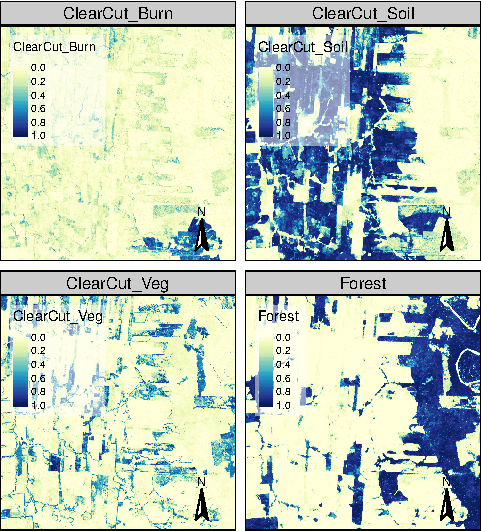
\includegraphics{Bayesian_smoothing_JSS_files/figure-latex/pcube-1} 

}

\caption[Class probabilities produced by random forest algorithm]{Class probabilities produced by random forest algorithm.}\label{fig:pcube}
\end{figure}
\end{CodeChunk}

The non-smoothed labelled map shows the need for post-processing. This map is obtained by taking the class of higher probability for each pixel as its label without considering the spatial context. This is done by \code{sits_label_classification()} whose main parameters are: (a) \code{cube}, a probability cube; (b) \code{output_dir}, directory for storing results; (c) \code{version}.

\begin{CodeChunk}
\begin{CodeInput}
R> label_cube_no_smooth <- sits_label_classification(
+     cube = probs_cube,
+     output_dir = tempdir,
+     version = "no_smooth")
\end{CodeInput}
\end{CodeChunk}

Figure \ref{fig:map1} shows the resulting map, which contains a significant number of outliers and misclassified pixels.

\begin{CodeChunk}
\begin{CodeInput}
R> plot(label_cube_no_smooth)
\end{CodeInput}
\begin{figure}[h]

{\centering 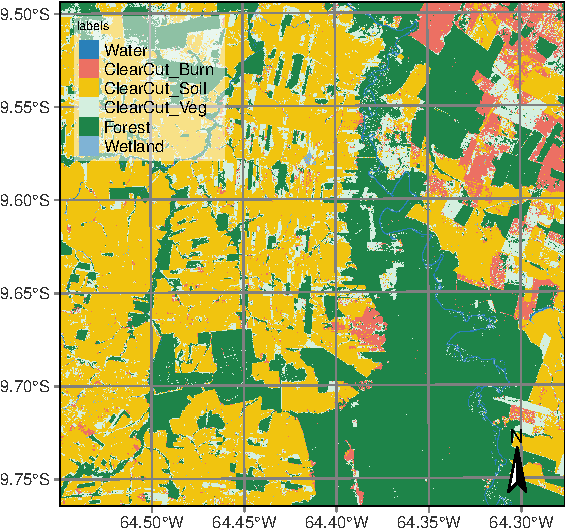
\includegraphics{Bayesian_smoothing_JSS_files/figure-latex/map1-1} 

}

\caption[Labelled map without smoothing]{Labelled map without smoothing.}\label{fig:map1}
\end{figure}
\end{CodeChunk}

\newpage

\hypertarget{estimating-the-local-logit-variances}{%
\subsection{Estimating the local logit variances}\label{estimating-the-local-logit-variances}}

The local logit variances correspond to the \(s^2_{i,k}\) parameter in the Bayesian inference and are estimated by \code{sits_variance()}. Its main parameters are: (a) \code{cube}, a probability cube; (b) \code{window_size}, dimension of the local neighbourhood; (c) \code{neigh_fraction}, the percentage of pixels in the neighbourhood used to calculate the variance; (d) \code{output_dir}, directory where results will be stored. The example below uses half of the pixels of a 7x7 window to estimate the variance. The chosen pixels will be those with the highest probability pixels to be more representative of the actual class distribution. The output values are the logit variances in the vicinity of each pixel.

\begin{CodeChunk}
\begin{CodeInput}
R> var_cube <- sits_variance(
+     cube = probs_cube,
+     window_size = 7,
+     neigh_fraction = 0.5,
+     output_dir = tempdir)
R> summary(var_cube, only_stats = TRUE)
\end{CodeInput}
\begin{CodeOutput}
 Water            ClearCut_Burn     ClearCut_Soil     ClearCut_Veg    
 Min.   : 0.000   Min.   : 0.0000   Min.   : 0.0000   Min.   : 0.000  
 1st Qu.: 0.090   1st Qu.: 0.0600   1st Qu.: 0.0700   1st Qu.: 0.110  
 Median : 1.560   Median : 0.1300   Median : 0.1700   Median : 0.400  
 Mean   : 2.302   Mean   : 0.3075   Mean   : 0.4994   Mean   : 1.213  
 3rd Qu.: 4.420   3rd Qu.: 0.2800   3rd Qu.: 0.4500   3rd Qu.: 1.280  
 Max.   :28.630   Max.   :12.5800   Max.   :20.8100   Max.   :24.690  
 Forest           Wetland          
 Min.   : 0.000   Min.   : 0.0000  
 1st Qu.: 0.060   1st Qu.: 0.0500  
 Median : 0.500   Median : 0.1200  
 Mean   : 1.847   Mean   : 0.4353  
 3rd Qu.: 3.030   3rd Qu.: 0.2800  
 Max.   :27.800   Max.   :12.4500  
\end{CodeOutput}
\end{CodeChunk}

The choice of the 7 x 7 window size is a compromise between having enough values to
estimate the parameters of a normal distribution and the need to capture local effects
for class patches of small sizes. Classes such as \code{Water} and \code{ClearCut_Burn}
tend to be spatially limited; a bigger window size could result in invalid values for
their respective normal distributions.

The summary statistics show that most local variance values are low, which is an expected result. Areas of low variance correspond to pixel neighbourhoods of high logit values for one the classes and low logit values for the others. High values of the local variances are relevant in areas of confusion between classes. Figure \ref{fig:vcube} shows the values of local logit variances for classes \code{ClearCut_Veg} and class \code{Forest}, considering only the 4th quartile of the distribution. Only the top 25\% of the values for each class are shown, emphasizing areas of high local variability.

\begin{CodeChunk}
\begin{CodeInput}
R> plot(var_cube, percentile = 0.75, labels = c("ClearCut_Veg", "Forest"))
\end{CodeInput}
\begin{figure}[h]

{\centering 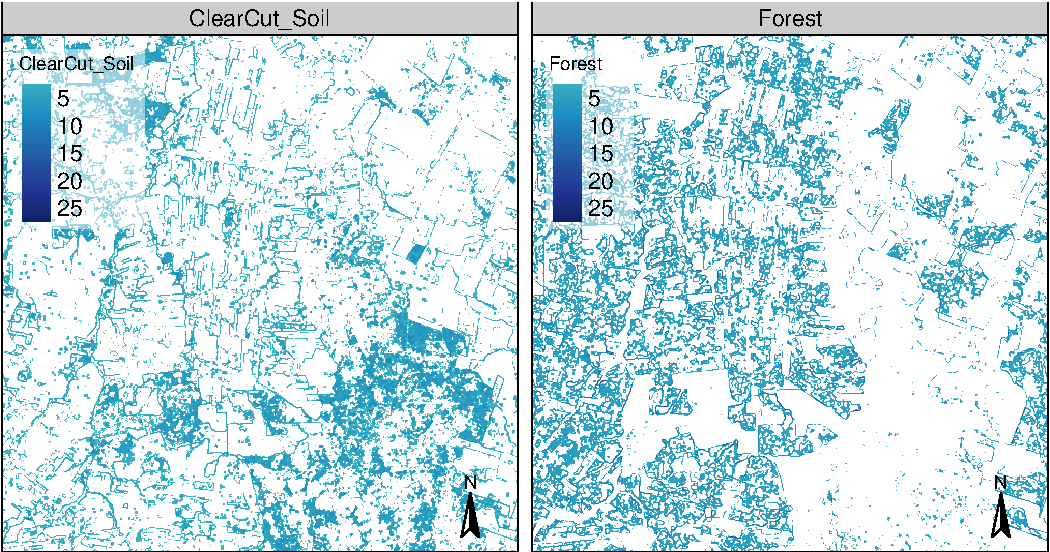
\includegraphics{Bayesian_smoothing_JSS_files/figure-latex/vcube-1} 

}

\caption[Logit variance map showing values above the 3rd quartile]{Logit variance map showing values above the 3rd quartile.}\label{fig:vcube}
\end{figure}
\end{CodeChunk}

Comparing the logit variance maps of Figure \ref{fig:vcube} with the probability maps of Figure \ref{fig:pcube} shows the relevance of expert knowledge. The areas of high probability of class \code{Forest} are mostly made of compact patches; areas of high local variance occur near the borders of these patches. By contrast, class \code{ClearCut_Veg} represents a transition between natural forest areas and places where all trees have been cut, which are associated to class \code{ClearCut_Soil}. Class \code{ClearCut_Veg} has a high spectral variability, since the extent of remaining vegetation after most trees have been removed is not uniform. For this reason, the local variance of class \code{ClearCut_Veg} is mostly patch-based, while that of class \code{Forest} is mostly border-based.

Further insights are provided by Figure \ref{fig:vhist} which shows the histograms of local variances per class. The values shown correspond to the 4th quartile (top 25\% of all values). The distribution of logit variances is uneven between the classes. Class \code{ClearCut_Veg} has a more balanced distribution, while most values in the 4th quartile of the \code{ClearCut_Soil} class have low values.

\begin{CodeChunk}
\begin{CodeInput}
R> plot(var_cube, type = "hist")
\end{CodeInput}
\begin{figure}[h]

{\centering 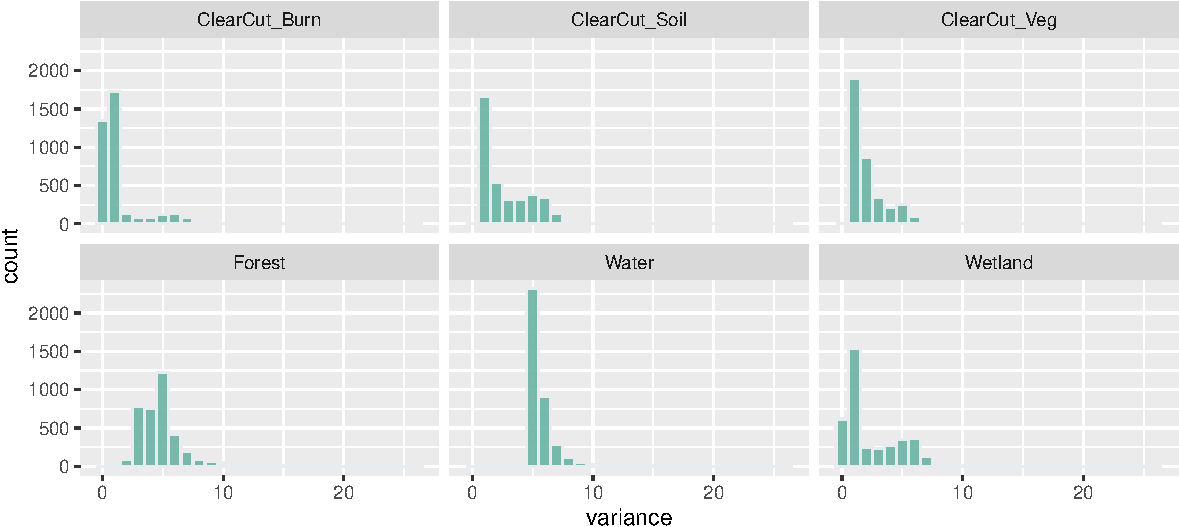
\includegraphics{Bayesian_smoothing_JSS_files/figure-latex/vhist-1} 

}

\caption[Histogram of top quartile of variances of class logits]{Histogram of top quartile of variances of class logits.}\label{fig:vhist}
\end{figure}
\end{CodeChunk}

\hypertarget{applying-bayesian-smoothing-to-remove-outliers}{%
\subsection{Applying Bayesian smoothing to remove outliers}\label{applying-bayesian-smoothing-to-remove-outliers}}

To remove the outliers in the classification map, \pkg{sits} uses \code{sits_smooth()}. Its main parameters are: (a) \code{cube}, a probability cube; (b) \code{window_size}, dimension of the local neighbourhood; (c) \code{neigh_fraction}, percentage of pixels in the neighbourhood used to calculate the variance; (d) \code{smoothness}, prior logit variances for each class; (e) \code{output_dir}, directory where results will be stored; (f) \code{version}, a string to distinguish different runs.

As discussed above, the effect of the Bayesian estimator depends on the values of the a priori variance \(\sigma^2_{k}\) set by the user and of the neighbourhood definition used to compute to local variance \(s^2_{i,1}\) for each pixel. To show the effects of different \(\sigma^2\) values we consider two cases: (a) setting \(\sigma^2\) to a high value close to the maximum value of local logit variance; (b) setting \(\sigma^2\) to a lower value close to the minimum value of the 4rd quartile.

\begin{CodeChunk}
\begin{CodeInput}
R> smooth_cube_high <- sits_smooth(
+     cube = probs_cube,
+     window_size = 7,
+     neigh_fraction = 0.5,
+     smoothness = c(25, 10, 20, 20, 25, 10),
+     output_dir = tempdir,
+     version = "smooth_high")
\end{CodeInput}
\end{CodeChunk}

The impact of Bayesian smoothing can be best captured by producing a labelled map using \code{sits_label_classification()} taking the smoothed image as its input. Figure \ref{fig:smth1} shows that the outliers and isolated pixels have been removed.

\begin{CodeChunk}
\begin{CodeInput}
R> label_cube_smooth_high <- sits_label_classification(
+     cube = smooth_cube_high,
+     output_dir = tempdir,
+     version = "smooth_high")
R> plot(label_cube_smooth_high)
\end{CodeInput}
\begin{figure}[h]

{\centering 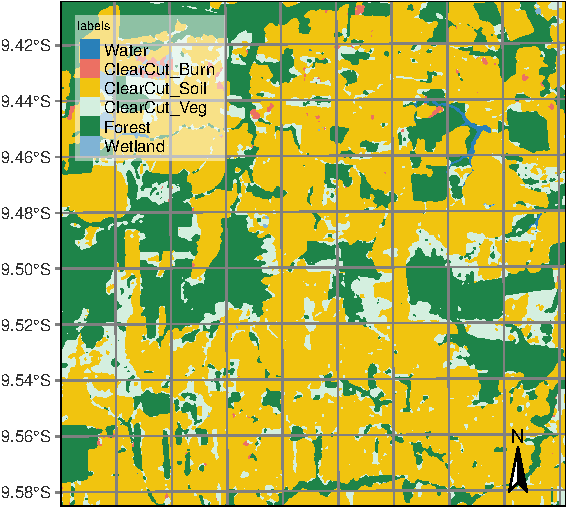
\includegraphics{Bayesian_smoothing_JSS_files/figure-latex/smth1-1} 

}

\caption[Labelled map with smoothing with high smoothness values]{Labelled map with smoothing with high smoothness values.}\label{fig:smth1}
\end{figure}
\end{CodeChunk}

In the smoothed map, the outliers have been removed by expanding forest areas. Forests have replaced small corridors of water and soil encircled by trees. This effect is due to the high probability of forest detection in the training data. Compare the smoothing with high values with the smoothing with values close to the minimum value of the 4th quartile of the local variance for each class, as computed below.

\begin{CodeChunk}
\begin{CodeInput}
R> smooth_cube_low <- sits_smooth(
+     cube = probs_cube,
+     window_size = 7,
+     neigh_fraction = 0.5,
+     smoothness = c(5, 1, 1, 2, 4, 1),
+     output_dir = tempdir,
+     version = "smooth_low")
\end{CodeInput}
\end{CodeChunk}

To see the impact of small \(\sigma^2\), we compute the labelled map.

\begin{CodeChunk}
\begin{CodeInput}
R> label_cube_smooth_low <- sits_label_classification(
+     cube = smooth_cube_low,
+     output_dir = tempdir,
+     version = "smooth_low")
R> plot(label_cube_smooth_low)
\end{CodeInput}
\begin{figure}[h]

{\centering 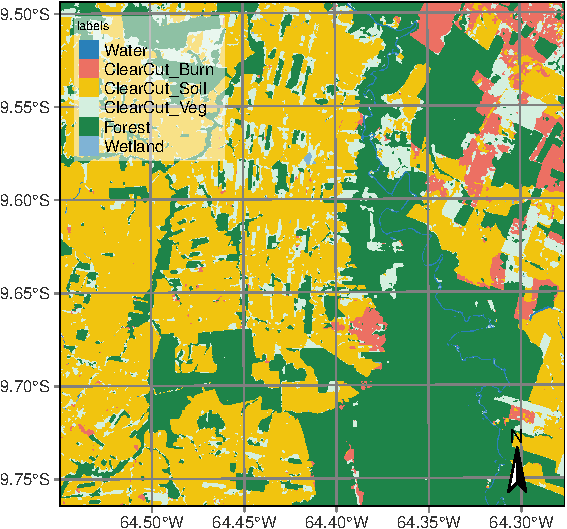
\includegraphics{Bayesian_smoothing_JSS_files/figure-latex/smth2-1} 

}

\caption[Labelled map with low smoothing parameters]{Labelled map with low smoothing parameters.}\label{fig:smth2}
\end{figure}
\end{CodeChunk}

A visual comparison between the two smoothed maps shows that there is an increase in the area of the \code{ClearCut_Veg} class. Such observation is confirmed by comparing the class areas of the non-smoothed map with the two types of smoothed maps, as shown below.

\begin{CodeChunk}
\begin{CodeInput}
R> sum1 <- summary(label_cube_no_smooth, only_stats = TRUE)
R> names(sum1) <- c("class", "area_k2_no_smooth")
R> sum2 <- summary(label_cube_smooth_high, only_stats = TRUE)
R> names(sum2) <- c("class", "area_k2_smooth_high")
R> sum3 <- summary(label_cube_smooth_low, only_stats = TRUE)
R> names(sum3) <- c("class", "area_k2_smooth_low")
R> dplyr::inner_join(sum1, sum2, by = "class") %>% 
+   dplyr::inner_join(sum3, by = "class")
\end{CodeInput}
\begin{CodeOutput}
          class area_k2_no_smooth area_k2_smooth_high area_k2_smooth_low
1         Water             1.767               1.030              1.106
2 ClearCut_Burn             7.743               2.043              2.771
3 ClearCut_Soil           215.400             234.500            224.700
4  ClearCut_Veg            65.350              47.620             57.470
5        Forest           105.100             112.500            111.200
6       Wetland             4.667               2.311              2.834
\end{CodeOutput}
\end{CodeChunk}

\hypertarget{relevance-of-expert-knowledge-in-bayesian-inference}{%
\subsection{Relevance of expert knowledge in Bayesian inference}\label{relevance-of-expert-knowledge-in-bayesian-inference}}

In the smoothed map with higher prior variance values, the most frequent classes (\code{ClearCut_Soil} and \code{Forest}) increased their areas at the expense of the others. As shown in Figure \ref{fig:pcube}, these classes occur in more compact patches than the others. In the second smoothed map, there is an increase in the area occupied by the \code{ClearCutVeg} class. This increase is due to the nature of this class, which represents a transition between a natural tropical area and one where all trees have been removed. Depending on the aims and practices of those responsible for deforestation, these areas may either have their tree cover removed completely. There are cases, however, where these places are abandoned and turn into secondary vegetation areas \cite{Uhl1988, Wang2020}.

This example shows the value of the Bayesian inference procedure compared with smoothing methods such as Gaussian and edge-aware filtering \citep{Schindler2012}. Most post-classification procedures use ad-hoc parameters which are not directly linked to the properties of the data. These parameters are based on the structure of the algorithm (e.g, size of the Gaussian kernel) and cannot easily be defined separately for each class. Bayesian inference allows the expert to control the output.

Based on the experience of the authors with different experts on land use classification, there are two main approaches for setting the \(\sigma^2_{k}\) parameter:

\begin{enumerate}
\def\labelenumi{\arabic{enumi}.}
\item
  To increase the neighbourhood influence compared with the probability values for each pixel, set the \(\sigma^2_{k}\) parameter with high values (20 or above) and increase the neighbourhood window size. Classes whose probabilities have strong spatial autocorrelation will tend to replace outliers.
\item
  To reduce the neighbourhood influence compared with the probabilities for each pixel of class \(k\), set the \(\sigma^2_{k}\) parameter with low values (5 or below) . In this way, classes with low spatial autocorrelation are more likely not to be relabelled.
\end{enumerate}

Consider the case of forest areas and watersheds. If an expert wishes to have compact areas classified as forests without many outliers inside them, she will set the \(\sigma^2\) parameter for the class ``Forest'' to be high. For comparison, to avoid that small watersheds with few similar neighbors being relabeled, it is advisable to avoid a strong influence of the neighbors, setting \(\sigma^2\) to be as low as possible. Therefore, choice of \(\sigma^2\) depends on the effect intended by the expert in the final classified map.

\hypertarget{comparison-with-other-methods}{%
\section{Comparison with other methods}\label{comparison-with-other-methods}}

\renewcommand\refname{Conclusion}
\bibliography{e-sensing.bib}



\end{document}
